\chapter{Design of the Adaptive Encryption Framework}
\label{chap:adaptive_framework}

\section{Design of the Adaptation Function}
\label{sec:adaptation_function}

The adaptation function $F: S(t) \rightarrow P(t)$ maps the observed communication state to a runtime cryptographic profile. In the broader architectural model, the state vector may include density, energy, packet loss, and threat level. For the executable prototype evaluated in this thesis, the effective switching rule is narrower and uses only threat and energy as direct inputs. This distinction is important: the chapter presents the architectural motivation first, then fixes the smaller state space that is actually implemented and benchmarked.

At the conceptual level, density is defined as
\begin{equation}
\rho(t) = \frac{n(t)}{A(t)},
\label{eq:density_time}
\end{equation}
where $n(t)$ is the number of active nodes and $A(t)$ is the covered area. The average energy level is
\begin{equation}
\bar{e}(t) = \frac{1}{n}\sum_{i=1}^{n} e_i(t),
\label{eq:avg_energy_time}
\end{equation}
and threat level is represented by $\theta(t) \in [0,1]$. In a full swarm deployment, packet loss $\lambda(t)$ and neighborhood dynamics would also inform profile selection. In the benchmark prototype, however, profile selection is reduced to threshold checks over $\bar{e}(t)$ and $\theta(t)$.

The benchmarked parameter vector is discrete:
\[
P(t) \in \{\text{heavy}, \text{balanced}, \text{lightweight}\}.
\]
These three profiles are defined as follows.
\begin{itemize}
  \item \textbf{Heavy}: AES-256-GCM for encryption and HMAC-SHA256 for additional data-plane authentication.
  \item \textbf{Balanced}: AES-192-GCM for encryption and HMAC-SHA256 for additional data-plane authentication.
  \item \textbf{Lightweight}: ChaCha20-Poly1305 for encryption and integrity, plus a sequence-bound hash token used as an inexpensive runtime authenticator.
\end{itemize}

The conceptual cost function remains
\begin{equation}
J = \alpha \cdot \tau(P) + \beta \cdot E(P) + \gamma \cdot R(S,P),
\label{eq:cost_function_adaptive}
\end{equation}
where $\tau(P)$ is latency, $E(P)$ is a platform-dependent energy term, and $R(S,P)$ is a residual-risk term. In this thesis, $J$ is used as a design lens rather than as a solved optimization problem. The practical benchmark does not claim to compute a globally optimal $P$; it validates that a threshold-based controller can switch among stronger and lighter profiles in a reproducible way.

The implemented decision rule is:
\begin{itemize}
  \item if $\theta \geq 0.8$, select the heavy profile;
  \item else if $\bar{e} \leq 0.2E_{\max}$, select the lightweight profile;
  \item else select the balanced profile.
\end{itemize}

Optimization-based and learned variants are possible extensions, but they are not implemented in the benchmark suite used in this work. The measured results later in the thesis therefore support claims about adaptive switching behavior, not about optimal profile selection.

\begin{figure}[H]
\centering
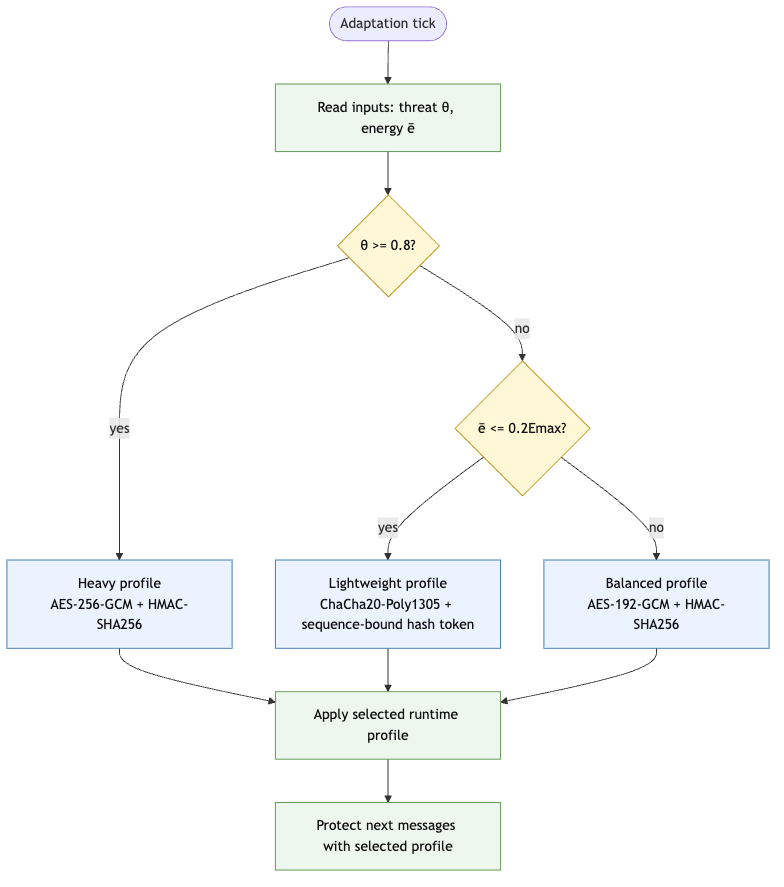
\includegraphics[width=\textwidth]{figs/adaptive_algorithm.png}
\caption{Adaptive cryptographic parameter selection algorithm.}
\label{fig:adaptive_algorithm}
\end{figure}

Figure~\ref{fig:adaptive_algorithm} should be read as an architectural diagram. The executable prototype instantiates its simplest branch: a threshold controller over threat and energy.

\section{Protocol Specification}
\label{sec:protocol_specification}

The protocol described in this thesis has two layers of scope. The first is the broader swarm-oriented architecture motivated by the literature. The second is the concrete pairwise prototype used in the practical evaluation. The practical evaluation validates only the second layer.

The \emph{initialization phase} of the prototype is pairwise. Peers are configured with a benchmark mode and a rekey interval, execute an X25519 key exchange, and derive epoch-specific material with HKDF-SHA256~\cite{rfc7748,rfc5869}. The resulting session keys are
\begin{equation}
k^{\mathrm{enc}}_{ij} = \mathrm{KDF}(K_{ij}, \text{``encryption''}),
\label{eq:kdf_enc}
\end{equation}
\begin{equation}
k^{\mathrm{mac}}_{ij} = \mathrm{KDF}(K_{ij}, \text{``authentication''}),
\label{eq:kdf_mac}
\end{equation}
where $K_{ij}$ is the X25519-derived shared secret. A fresh exchange is repeated on rekey events so that each epoch uses newly derived material. This supports compromise containment at the epoch level. The benchmark does not implement signed bootstrap announcements or signed configuration updates, so the practical evaluation should not be interpreted as validating control-plane authenticity.

The \emph{operational phase} protects each message with the currently selected runtime profile. For message transmission, the sender generates a nonce $N$ and encrypts plaintext $m$ as
\begin{equation}
c = \mathrm{Enc}\!\left(k^{\mathrm{enc}}_{ij}, N, m\right).
\label{eq:encrypt_msg}
\end{equation}
The transmitted packet format depends on the active profile.
\begin{itemize}
  \item In the heavy and balanced profiles, the packet carries $\{N, c, \sigma\}$ where $\sigma=\mathrm{MAC}(k^{\mathrm{mac}}_{ij}, N \Vert c)$.
  \item In the lightweight profile, the packet carries $\{N, c, h_i\}$ where $h_i$ is the sequence-bound hash token associated with the current epoch and message sequence number.
\end{itemize}
Upon reception, the receiver verifies the profile-appropriate authenticator, rejects already accepted sequence numbers within the current epoch, and decrypts only if verification succeeds.

The \emph{adaptation phase} is also pairwise in the prototype. At each adaptation interval, the sender reads the current threat and energy inputs from the active scenario, applies the threshold rule, and chooses one of the three runtime profiles. The benchmark does not implement gossip-based aggregation, leader election, or consensus-based synchronized switching across many nodes. Those mechanisms remain architectural extensions for a future multi-peer implementation.

The main loop can be summarized as follows:

\begin{lstlisting}
Initialization:
  Generate X25519 key pair
  Perform pairwise key exchange
  Derive epoch keys via HKDF
  Set initial profile P <- balanced

Operational loop:
  Every T_adapt seconds:
    Read current threat and energy inputs
    Compute P_new <- F(threat, energy)
    If P_new != P:
      Switch runtime profile: P <- P_new

  On sending message m:
    Generate nonce N
    Encrypt per selected profile
    Attach HMAC or hash token
    Transmit packet

  On receiving packet:
    Verify profile-appropriate authenticator
    If verification succeeds:
      Decrypt and process
    Else:
      Drop packet
\end{lstlisting}

This specification is intentionally narrower than a full swarm-control-plane protocol. It is, however, sufficient for the benchmarked claim of this thesis: a pairwise adaptive secure-communication prototype can be implemented, switched between profiles, and measured under constrained execution.

\section{Parameter Selection Algorithm}
\label{sec:parameter_selection}

For the executable benchmark, the input metrics of the selector are intentionally minimal. The implemented state vector is
\[
S = (\bar{e}, \theta),
\]
and the parameter vector is
\[
P = (\text{profile}).
\]
The rekey interval is fixed by the benchmark scenario rather than chosen by the decision tree; the selector itself returns only the runtime profile.
The profile selection rule is piecewise constant:
\[
F(S) =
\begin{cases}
\text{heavy}, & \theta \geq 0.8 \\
\text{lightweight}, & \bar{e} \leq 0.2E_{\max} \\
\text{balanced}, & \text{otherwise.}
\end{cases}
\]

This rule is simple by design. It is sufficient to demonstrate two qualitatively important behaviors:
\begin{itemize}
  \item escalation into a stronger profile when threat is high;
  \item degradation into a lighter profile when energy is low.
\end{itemize}

Several quantities mentioned earlier in the architectural model are not part of the implemented selector. Density $\rho$, packet loss $\lambda$, and mission criticality $\kappa$ remain relevant design variables, but they are not direct switching inputs in the current code base. Their role in this chapter is therefore motivational rather than experimental.

Threshold values are fixed manually for the benchmark:
\[
\theta_{\mathrm{crit}} = 0.8, \qquad E_{\mathrm{crit}} = 0.2E_{\max}.
\]
The benchmark scenarios are chosen to exercise these thresholds directly. A richer implementation could calibrate them from historical data, simulation traces, or online learning, but those extensions are outside the validated scope of the present prototype.

\begin{figure}[H]
\centering

\includegraphics[width=\textwidth]{parameter_selection_flowchart.png}
\caption{Decision-tree-based algorithm for adaptive cryptographic parameter selection.}
\label{fig:parameter_selection}
\end{figure}

Figure~\ref{fig:parameter_selection} should therefore be interpreted as a simplified decision tree for the current prototype, not as a proof of global optimality.

\section{Implementation Aspects}
\label{sec:implementation_aspects}

The benchmark implementation targets a constrained but host-based execution environment. It uses Docker containers and gRPC-connected peers to emulate runtime isolation, while CPU and memory limits approximate weaker embedded hardware. The practical measurements therefore say more about software behavior under constrained execution than about the exact latency of a deployed robotic platform.

The prototype is pairwise on the measured data path. Even when a scenario file specifies more than two peers, the current benchmark focuses on the primary \texttt{peer\_a} $\rightarrow$ \texttt{peer\_b} exchange and does not claim to validate multi-hop routing, neighborhood churn, or consensus traffic. That choice keeps the benchmark reproducible and makes profile-switching behavior easy to inspect, but it also bounds the external validity of the results.

The overhead of adaptation in this prototype is negligible relative to packet protection because profile selection is a threshold check. The more meaningful costs are rekeying, data-plane protection, and queueing under CPU pressure. For that reason, the practical evaluation chapter focuses on latency, throughput, switching behavior, and a model-based energy proxy rather than on the controller itself.

Implementation guidance remains conventional. Secure random generation is required for key exchange and nonce creation; constant-time cryptographic libraries remain desirable; and any future extension toward a field-ready system would need a genuine authenticated control plane, device identity management, and deployment-specific fault handling~\cite{chenSecuringEmergentBehaviour2021}. New lightweight standards such as Ascon may also be relevant for future constrained-device variants, but they are not part of the implemented benchmark profile set~\cite{nistSP800232Ascon}.
